%%%%%%%%%%%%%%%%%%%%%%%%%%%%%%%%%%%%%%%%%%%%%%%%%%%%%%%%%%%%%%%%%%%%%%%%%%%
%%
%%  ch-resol.tex
%%
%%  Created: Fri Oct 10 14:24:37 1997
%%  Author.: Jose Carlos Gonzales
%%  Notes..:
%%          
%%-------------------------------------------------------------------------
%% Filename: $RCSfile$
%% Revision: $Revision$
%% Date:     $Date$
%%%%%%%%%%%%%%%%%%%%%%%%%%%%%%%%%%%%%%%%%%%%%%%%%%%%%%%%%%%%%%%%%%%%%%%%%%%


\def\SIZE{\mbox{\scshape size}\xspace}
\def\LENGTH{\mbox{\scshape length}\xspace}
\def\WIDTH{\mbox{\scshape width}\xspace}
\def\DISTANCE{\mbox{\scshape distance}\xspace}

\chapter{Angular and Energetic Resolutions in \MAGIC}
\label{chapter:resol}

\section{The Angular Resolution}

\section{The Energy Resolution}

In order to develop theories and discriminate between different models
for acceleration, emission, absorption and propagation of very high
energy particle, a good knowledge of the spectra of the detected
cosmic and $\gamma$-rays is needed.

One of the most important parameters of any given detector is its the
energy resolution.  In the case of Imaging Atmospheric Cherenkov
telescopes (IACTs), the evaluation of this parameter has to be done by
using Monte Carlo methods.  As we have seen, the energy of the primary
particles is not measured directly: primary particles entering the
atmosphere initiate a shower of secondary particles, including
\Cherenkov photons, which can be used to estimate the energy of the
the initial particle.

Currently, existing IACTs have a lower detection energy of
$\geq$200\u{GeV}.  In earlier works (see \cite{MAGIC:Gonzalez_Kruger})
it has been shown for the first time that one can design large IACTs
which allow us to dramatically lower the energy threshold and to
measure successfully at energies above 10\u{GeV} \cite{MAGIC:DR}.

\begin{figure}[t]
\centering
a)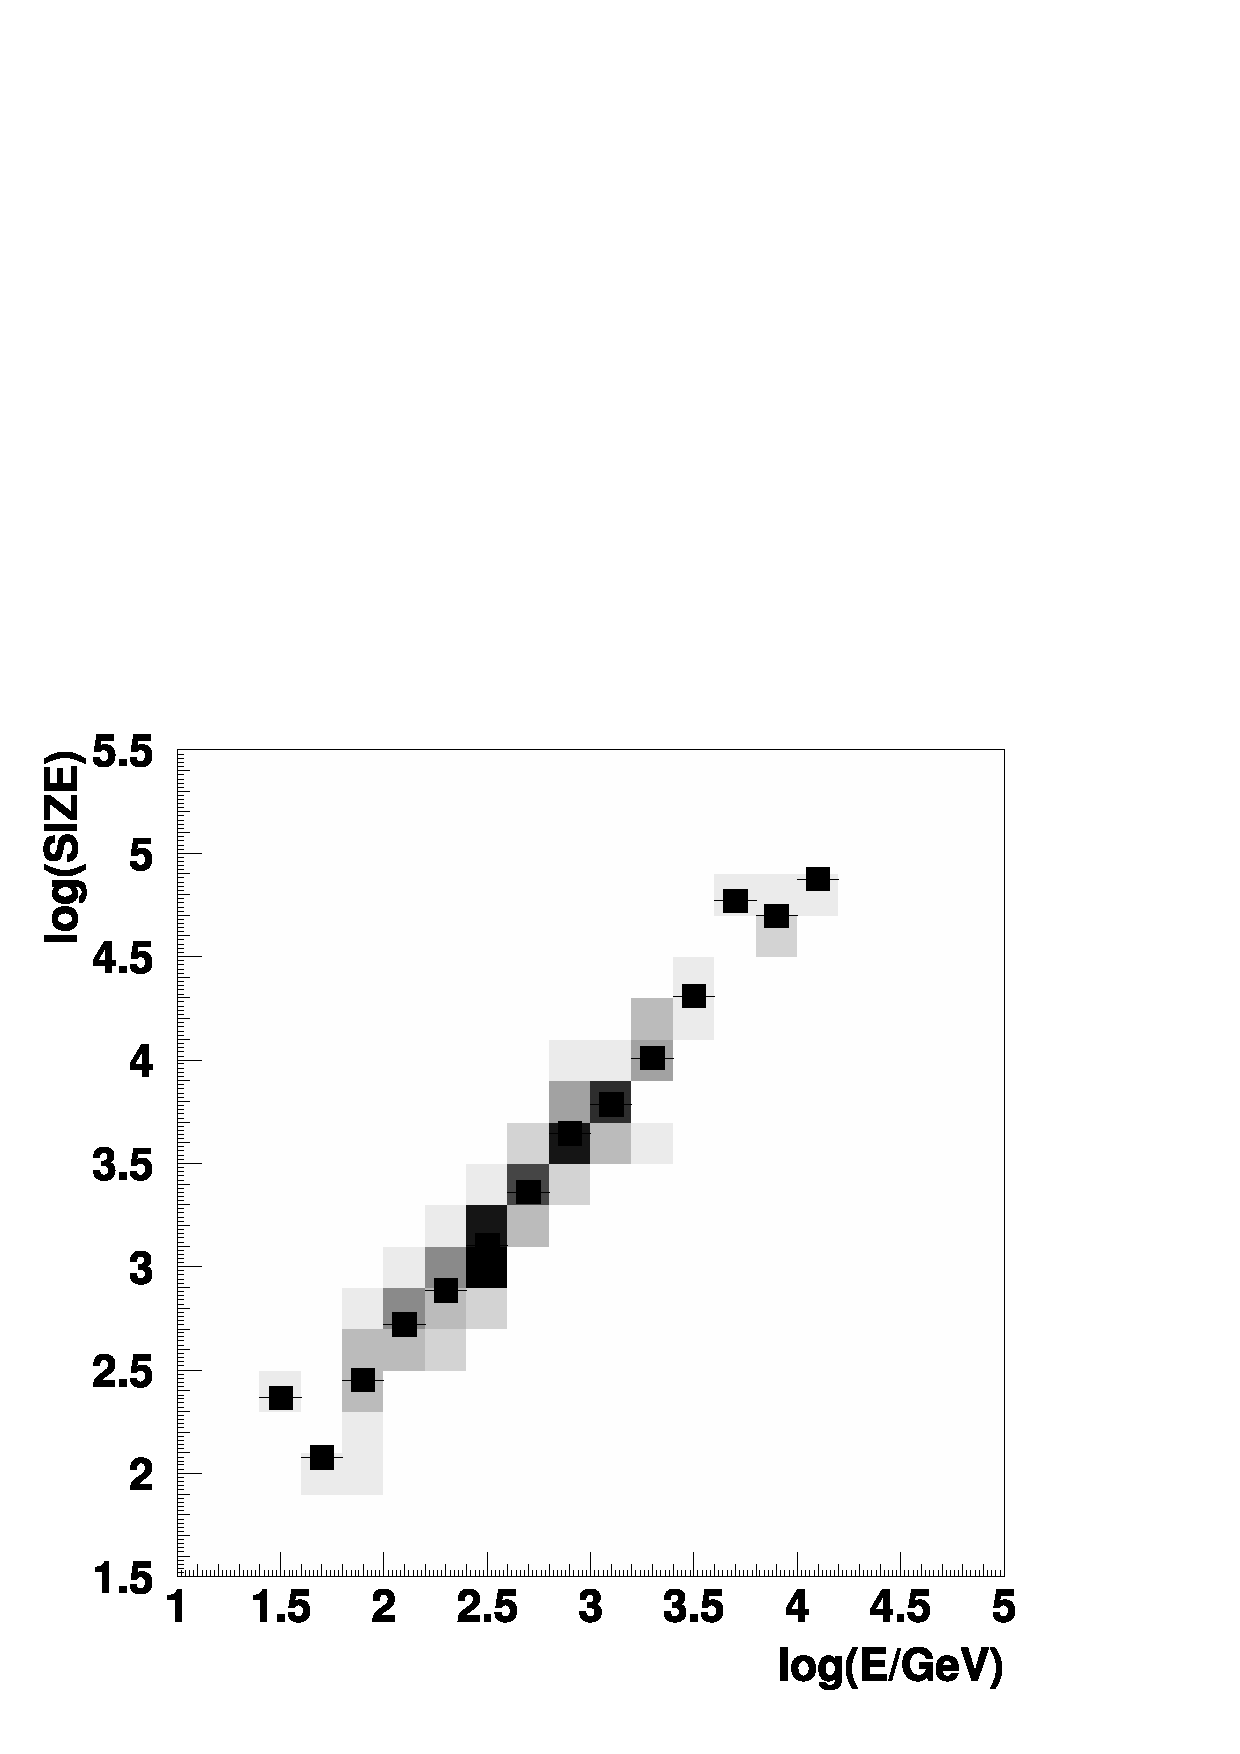
\includegraphics[width=0.42\linewidth]{lza0509dist-a}
\hfil
b)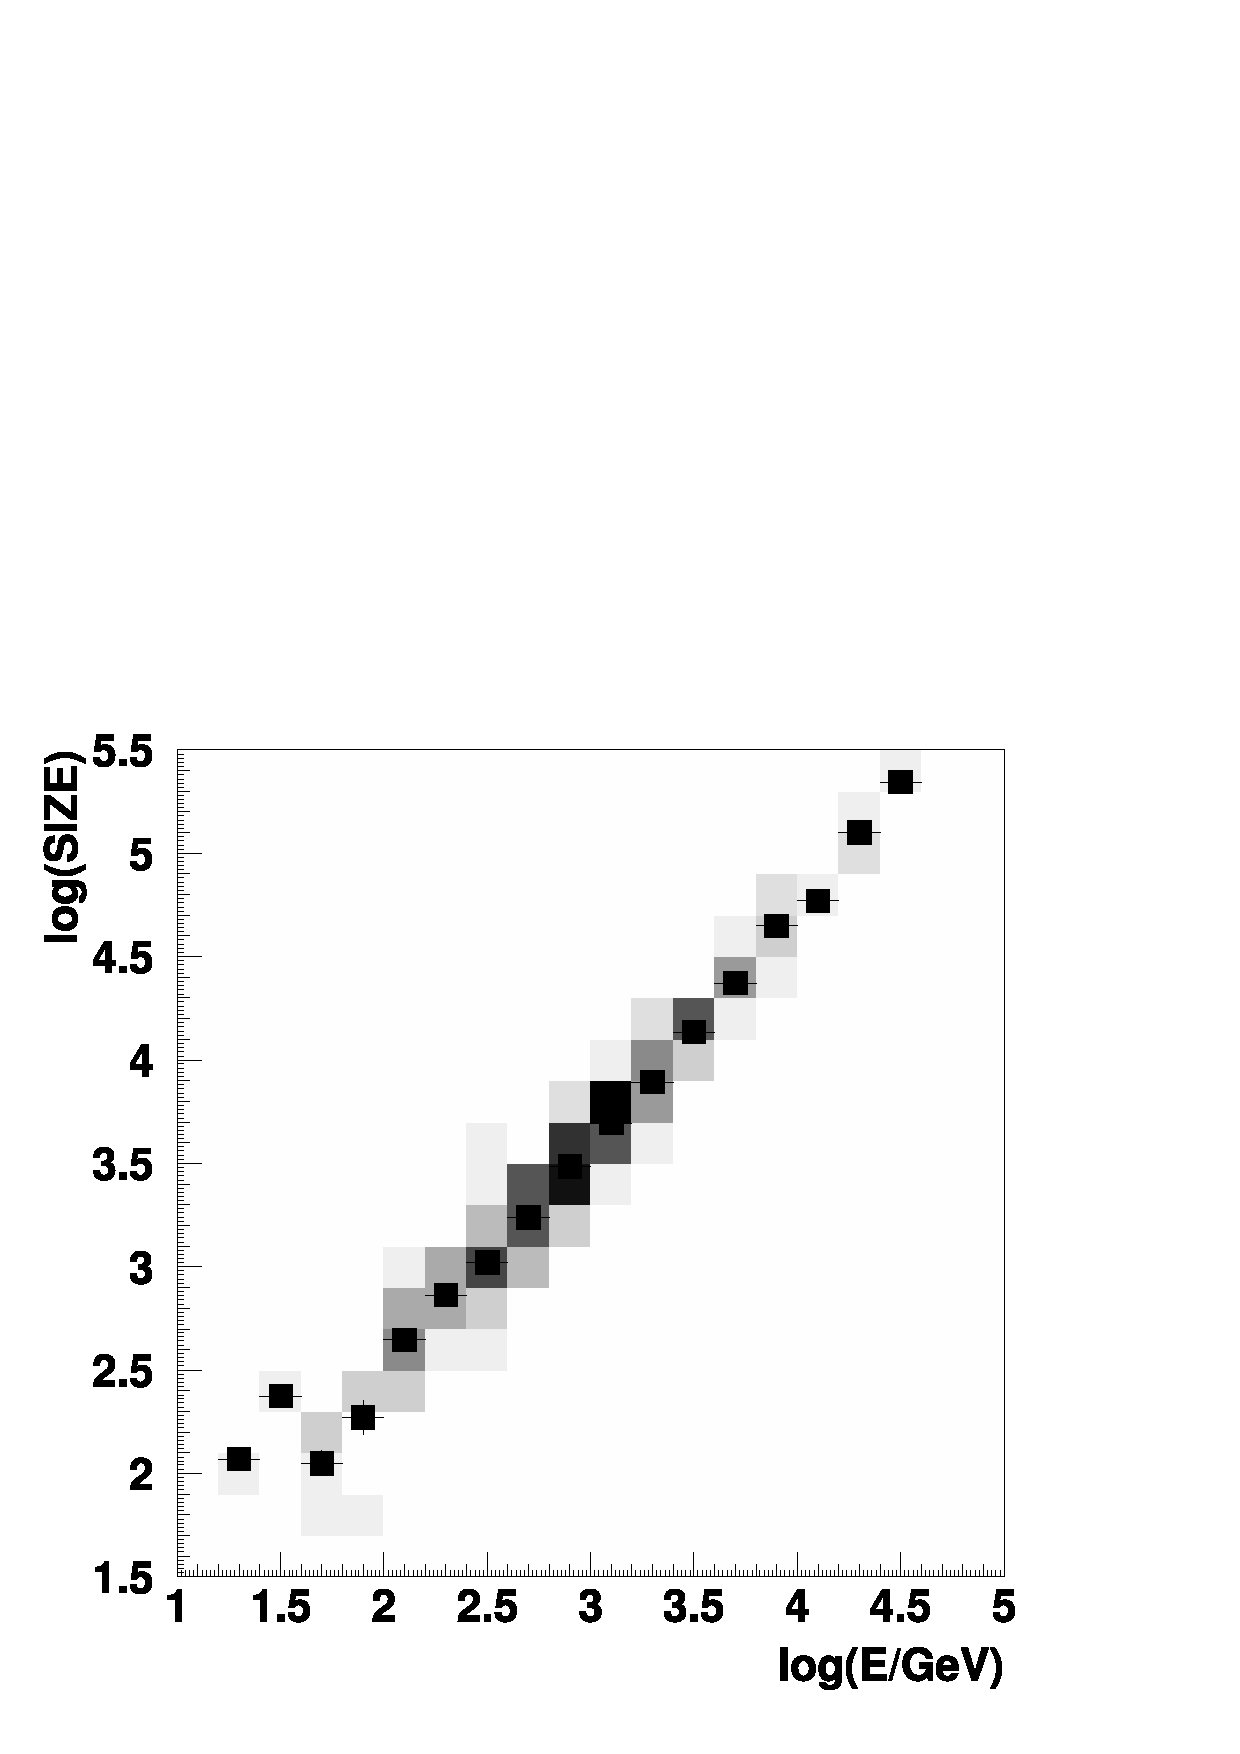
\includegraphics[width=0.42\linewidth]{hza0509dist-a}
\caption{\label{logSIZElogE:fig}
  Total amount of light in the camera of MAGIC as a function of the
  energy of the primary, for those events passing the cuts applied for
  the \DISTANCE range 0.5\deg -- 0.9\deg, and for the zenith angle
  ranges: a) $\cos\theta>0.96$ (approx.  $5\deg \leq \theta \leq
  16\deg$); and b) $\cos\theta<0.96$ (approx. $16\deg \leq \theta \leq
  25\deg$).}  \vskip -15pt
\end{figure}

In order to estimate the energy of the primary of an atmospheric
shower, several parameters have to be taken into account, being the
most important the impact parameter and zenith angle of the shower,
the total amount of light, and the position of the maximum development
in the atmosphere, $h_{\mathrm{max}}$:
%
\begin{equation}
E = E(\SIZE, \rho_{\mathrm{impact}},
\theta_{\mathrm{zenith}}; h_{\mathrm{max}}; \WIDTH, \LENGTH, \ldots)
\end{equation}
%
We use the total amount of light in the camera of MAGIC as an
observable directly correlated with the total amount of light, and
hence with the energy of the shower. In our studies, a simplification
of this model has been used:
%
\begin{equation}
E = E(\SIZE, \DISTANCE^{\mathrm{bins}},
\theta_{\mathrm{zenith}}^{\mathrm{bins}})
\label{simple.eq}
\end{equation}
%
Additional, second-order parameters are also correlated with the
energy of the primary, but these fine effects are not yet taken into
account. Further studies are in progress.

In Fig. \ref{logSIZElogE:fig} we show the amount of light in the
camera of MAGIC for one of the studied slices in \DISTANCE, namely
0.5\deg -- 0.9\deg, after all the cuts were applied.  We can see that
the amount of light measured is not univocally determined by the
energy of the primary. First, the density of light not exactly
constant with the impact parameter; second, the binning in zenith
angle ($\cos\theta>0.96$ and $\cos\theta<0.96$ in this case) affects
in the same way; also are important the effects of a restricted
trigger region in the camera, and the finite camera size itself; and
last, but not least, the fluctuations on the shower itself, which are
completely unavoidable: for a fixed impact parameter, zenith angle and
energy of the primary, still the shower can develop deeper of earlier
in the atmosphere, and this results in a fluctuation in the amount and
density of light in the detector level.

\begin{figure}[t]
\centering
a)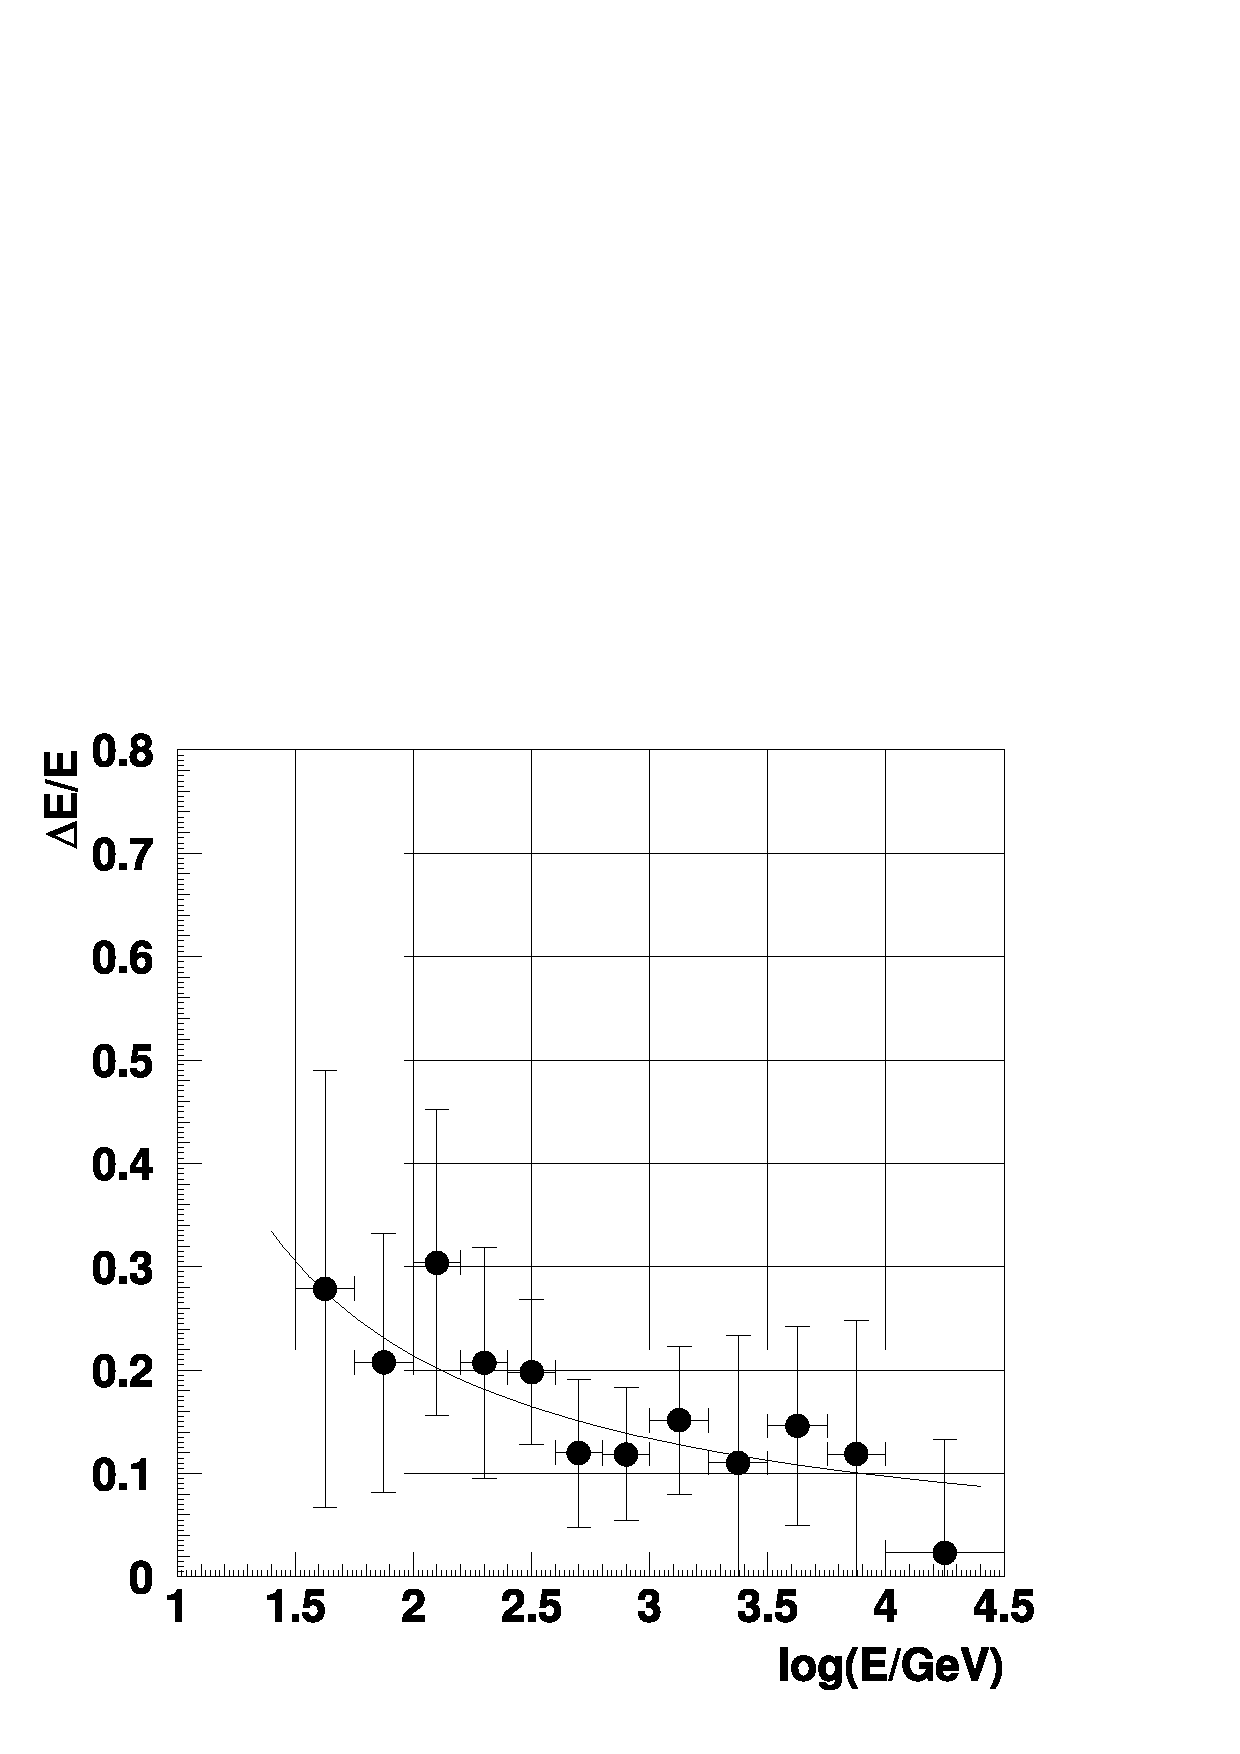
\includegraphics[width=0.42\linewidth]{lza0509dist-b}
\hfil
b)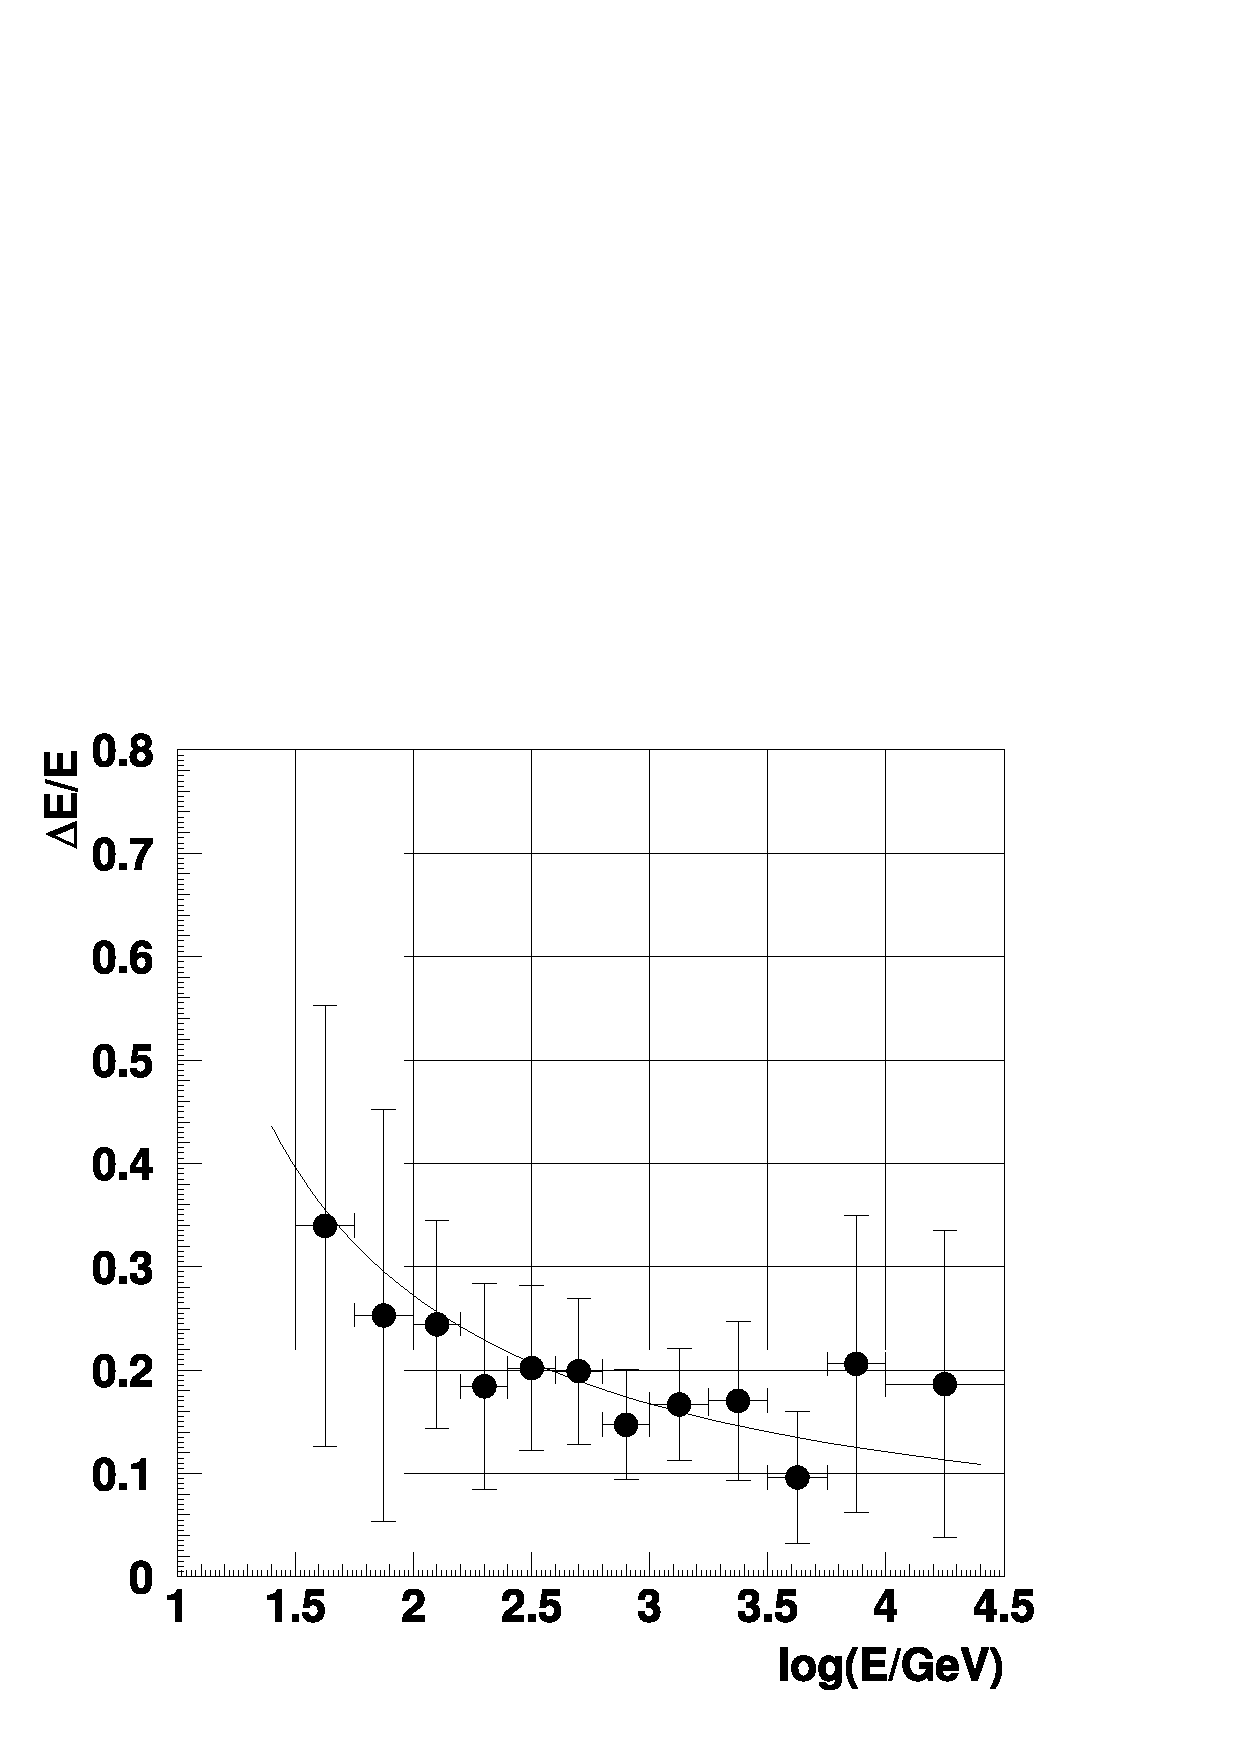
\includegraphics[width=0.42\linewidth]{hza0509dist-b}
\caption{\label{resolutions:fig}
  Calculated energy resolution for the cases a) and b) of the Fig.
  \protect\ref{logSIZElogE:fig}.}
\vskip -15pt
\end{figure}

As we can see in Fig.  \ref{logSIZElogE:fig}, however, in the mean the
amount of light is strongly correlated over almost three order of
magnitude in energy with the energy of the primary (under the
necessary restrictions in impact parameter, i.e. \DISTANCE, and zenith
angle).  This correlation allows one to estimate the energy of the
primary.  The energy resolution, i.e., the mean error that we can make
in this prediction of the primary energy, is shown in Fig.
\ref{resolutions:fig}, were we plot the energy resolution $\Delta E/E$
obtained for the same sets used in Fig.  \ref{logSIZElogE:fig}. As we
see, for the case of $\cos\theta>0.96$, MAGIC reaches a value of about
$\leq$15\% at energies above 300\u{GeV}. This value is worse, around
30\%, for low energies, near the threshold (around 30-40\u{GeV} for
the PMTs camera), where we are affected by the trigger bias (events
trigger due to positive fluctuations), but improves to less 15\%
around several \u{TeV}, getting close to 10\% for energies of tenths
of \u{TeV}.  Our studies indicate that for the case $\cos\theta<0.96$
a mean value of 20\% is easily reachable.  Note that these results are
obtained with the simple approach expressed by Eq.  \ref{simple.eq}.

\section{Other methods for angular and energy resolution estimation}

\endinput
%
%% Local Variables:
%% mode:latex
%% End:

%%EOF
